% =====================================================================
% Abbildung: Traceability-Matrix für den Indoor-Roboter (Auszug)
% Passend zu Kapitel 20, Abschnitt "Traceability-Matrix"
%
% Einbindung im Buch, z. B. in chapters/20_traceability.tex:
%
%   \begin{figure}[H]
%     \centering
%     % =====================================================================
% Abbildung: Traceability-Matrix für den Indoor-Roboter (Auszug)
% Passend zu Kapitel 20, Abschnitt "Traceability-Matrix"
%
% Einbindung im Buch, z. B. in chapters/20_traceability.tex:
%
%   \begin{figure}[H]
%     \centering
%     % =====================================================================
% Abbildung: Traceability-Matrix für den Indoor-Roboter (Auszug)
% Passend zu Kapitel 20, Abschnitt "Traceability-Matrix"
%
% Einbindung im Buch, z. B. in chapters/20_traceability.tex:
%
%   \begin{figure}[H]
%     \centering
%     % =====================================================================
% Abbildung: Traceability-Matrix für den Indoor-Roboter (Auszug)
% Passend zu Kapitel 20, Abschnitt "Traceability-Matrix"
%
% Einbindung im Buch, z. B. in chapters/20_traceability.tex:
%
%   \begin{figure}[H]
%     \centering
%     \input{figures/fig_kap20_traceability_matrix}
%     \caption{Auszug aus einer Traceability-Matrix: Jede Zeile verbindet
%       eine Anforderung über Funktion, Systemelement und ROS2-Node bis
%       zum Testfall.}
%     \label{fig:kap20-traceability-matrix}
%   \end{figure}
%
% Benoetigte Pakete (im Buch bereits in main.tex geladen): tikz
% Benoetigte TikZ-Bibliotheken: positioning, arrows.meta, shadows, calc
% =====================================================================

\input{figures/fig_kap20_traceability_matrix.tikz}

%     \caption{Auszug aus einer Traceability-Matrix: Jede Zeile verbindet
%       eine Anforderung über Funktion, Systemelement und ROS2-Node bis
%       zum Testfall.}
%     \label{fig:kap20-traceability-matrix}
%   \end{figure}
%
% Benoetigte Pakete (im Buch bereits in main.tex geladen): tikz
% Benoetigte TikZ-Bibliotheken: positioning, arrows.meta, shadows, calc
% =====================================================================

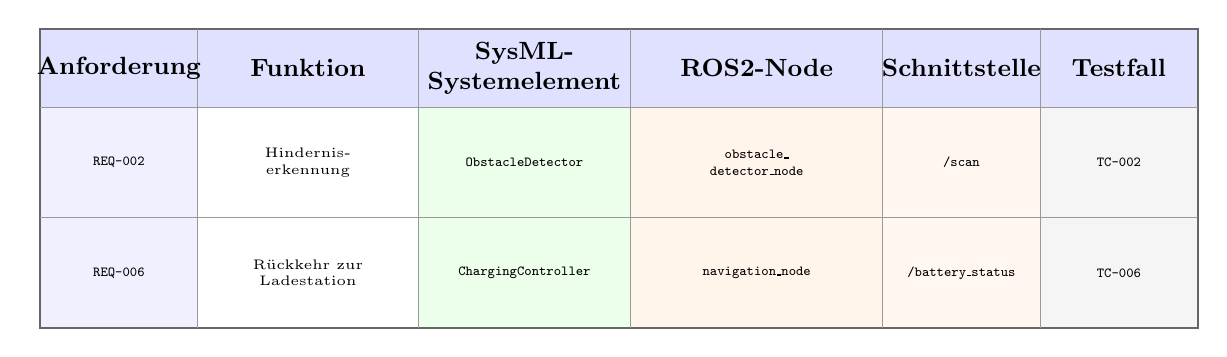
\begin{tikzpicture}[
    every node/.style={font=\small},
    x=1cm, y=1cm
]

% --- Spaltengrenzen (x) und Zeilengrenzen (y) in cm ---
% Spalten: Anforderung | Funktion | SysML-Systemelement | ROS2-Node | Schnittstelle | Testfall
% x0=0, x1=2.0, x2=4.8, x3=7.5, x4=10.7, x5=12.7, x6=14.7
% Zeilen (von oben): y0=3.8 (Kopf oben), y1=2.8 (Kopf unten / Zeile1 oben),
%                     y2=1.4 (Zeile1 unten / Zeile2 oben), y3=0 (Zeile2 unten)

% --- Spaltenhintergrund fuer Datenzeilen (y3 bis y1) ---
\fill[blue!6]   (0,0)    rectangle (2.0,2.8);
\fill[white]    (2.0,0)  rectangle (4.8,2.8);
\fill[green!8]  (4.8,0)  rectangle (7.5,2.8);
\fill[orange!8] (7.5,0)  rectangle (10.7,2.8);
\fill[orange!6] (10.7,0) rectangle (12.7,2.8);
\fill[black!4]  (12.7,0) rectangle (14.7,2.8);

% --- Kopfzeile ueberdeckend einfaerben ---
\fill[blue!12] (0,2.8) rectangle (14.7,3.8);

% --- Rasterlinien: Aussenrahmen ---
\draw[black!60, thick] (0,0) rectangle (14.7,3.8);

% --- Rasterlinien: senkrechte Spaltentrenner ---
\draw[black!40] (2.0,0)  -- (2.0,3.8);
\draw[black!40] (4.8,0)  -- (4.8,3.8);
\draw[black!40] (7.5,0)  -- (7.5,3.8);
\draw[black!40] (10.7,0) -- (10.7,3.8);
\draw[black!40] (12.7,0) -- (12.7,3.8);

% --- Rasterlinien: waagrechte Zeilentrenner ---
\draw[black!40] (0,1.4) -- (14.7,1.4);
\draw[black!40] (0,2.8) -- (14.7,2.8);

% --- Kopfzeilentext ---
\node[font=\small\bfseries] at (1.0,3.3)  {Anforderung};
\node[font=\small\bfseries] at (3.4,3.3)  {Funktion};
\node[font=\small\bfseries, align=center] at (6.15,3.3) {SysML-\\Systemelement};
\node[font=\small\bfseries] at (9.1,3.3)  {ROS2-Node};
\node[font=\small\bfseries] at (11.7,3.3) {Schnittstelle};
\node[font=\small\bfseries] at (13.7,3.3) {Testfall};

% --- Zeile 1: REQ-002 ---
\node[font=\tiny] at (1.0,2.1)  {\texttt{REQ-002}};
\node[font=\tiny, align=center] at (3.4,2.1)  {Hindernis-\\erkennung};
\node[font=\tiny] at (6.15,2.1) {\texttt{ObstacleDetector}};
\node[font=\tiny, align=center] at (9.1,2.1)  {\texttt{obstacle\_}\\\texttt{detector\_node}};
\node[font=\tiny] at (11.7,2.1) {\texttt{/scan}};
\node[font=\tiny] at (13.7,2.1) {\texttt{TC-002}};

% --- Zeile 2: REQ-006 ---
\node[font=\tiny] at (1.0,0.7)  {\texttt{REQ-006}};
\node[font=\tiny, align=center] at (3.4,0.7)  {Rückkehr zur\\Ladestation};
\node[font=\tiny] at (6.15,0.7) {\texttt{ChargingController}};
\node[font=\tiny] at (9.1,0.7)  {\texttt{navigation\_node}};
\node[font=\tiny] at (11.7,0.7) {\texttt{/battery\_status}};
\node[font=\tiny] at (13.7,0.7) {\texttt{TC-006}};

\end{tikzpicture}


%     \caption{Auszug aus einer Traceability-Matrix: Jede Zeile verbindet
%       eine Anforderung über Funktion, Systemelement und ROS2-Node bis
%       zum Testfall.}
%     \label{fig:kap20-traceability-matrix}
%   \end{figure}
%
% Benoetigte Pakete (im Buch bereits in main.tex geladen): tikz
% Benoetigte TikZ-Bibliotheken: positioning, arrows.meta, shadows, calc
% =====================================================================

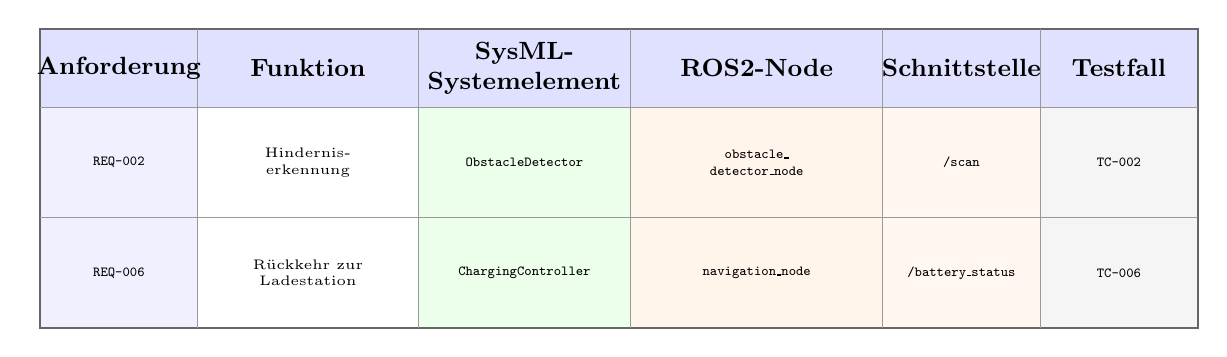
\begin{tikzpicture}[
    every node/.style={font=\small},
    x=1cm, y=1cm
]

% --- Spaltengrenzen (x) und Zeilengrenzen (y) in cm ---
% Spalten: Anforderung | Funktion | SysML-Systemelement | ROS2-Node | Schnittstelle | Testfall
% x0=0, x1=2.0, x2=4.8, x3=7.5, x4=10.7, x5=12.7, x6=14.7
% Zeilen (von oben): y0=3.8 (Kopf oben), y1=2.8 (Kopf unten / Zeile1 oben),
%                     y2=1.4 (Zeile1 unten / Zeile2 oben), y3=0 (Zeile2 unten)

% --- Spaltenhintergrund fuer Datenzeilen (y3 bis y1) ---
\fill[blue!6]   (0,0)    rectangle (2.0,2.8);
\fill[white]    (2.0,0)  rectangle (4.8,2.8);
\fill[green!8]  (4.8,0)  rectangle (7.5,2.8);
\fill[orange!8] (7.5,0)  rectangle (10.7,2.8);
\fill[orange!6] (10.7,0) rectangle (12.7,2.8);
\fill[black!4]  (12.7,0) rectangle (14.7,2.8);

% --- Kopfzeile ueberdeckend einfaerben ---
\fill[blue!12] (0,2.8) rectangle (14.7,3.8);

% --- Rasterlinien: Aussenrahmen ---
\draw[black!60, thick] (0,0) rectangle (14.7,3.8);

% --- Rasterlinien: senkrechte Spaltentrenner ---
\draw[black!40] (2.0,0)  -- (2.0,3.8);
\draw[black!40] (4.8,0)  -- (4.8,3.8);
\draw[black!40] (7.5,0)  -- (7.5,3.8);
\draw[black!40] (10.7,0) -- (10.7,3.8);
\draw[black!40] (12.7,0) -- (12.7,3.8);

% --- Rasterlinien: waagrechte Zeilentrenner ---
\draw[black!40] (0,1.4) -- (14.7,1.4);
\draw[black!40] (0,2.8) -- (14.7,2.8);

% --- Kopfzeilentext ---
\node[font=\small\bfseries] at (1.0,3.3)  {Anforderung};
\node[font=\small\bfseries] at (3.4,3.3)  {Funktion};
\node[font=\small\bfseries, align=center] at (6.15,3.3) {SysML-\\Systemelement};
\node[font=\small\bfseries] at (9.1,3.3)  {ROS2-Node};
\node[font=\small\bfseries] at (11.7,3.3) {Schnittstelle};
\node[font=\small\bfseries] at (13.7,3.3) {Testfall};

% --- Zeile 1: REQ-002 ---
\node[font=\tiny] at (1.0,2.1)  {\texttt{REQ-002}};
\node[font=\tiny, align=center] at (3.4,2.1)  {Hindernis-\\erkennung};
\node[font=\tiny] at (6.15,2.1) {\texttt{ObstacleDetector}};
\node[font=\tiny, align=center] at (9.1,2.1)  {\texttt{obstacle\_}\\\texttt{detector\_node}};
\node[font=\tiny] at (11.7,2.1) {\texttt{/scan}};
\node[font=\tiny] at (13.7,2.1) {\texttt{TC-002}};

% --- Zeile 2: REQ-006 ---
\node[font=\tiny] at (1.0,0.7)  {\texttt{REQ-006}};
\node[font=\tiny, align=center] at (3.4,0.7)  {Rückkehr zur\\Ladestation};
\node[font=\tiny] at (6.15,0.7) {\texttt{ChargingController}};
\node[font=\tiny] at (9.1,0.7)  {\texttt{navigation\_node}};
\node[font=\tiny] at (11.7,0.7) {\texttt{/battery\_status}};
\node[font=\tiny] at (13.7,0.7) {\texttt{TC-006}};

\end{tikzpicture}


%     \caption{Auszug aus einer Traceability-Matrix: Jede Zeile verbindet
%       eine Anforderung über Funktion, Systemelement und ROS2-Node bis
%       zum Testfall.}
%     \label{fig:kap20-traceability-matrix}
%   \end{figure}
%
% Benoetigte Pakete (im Buch bereits in main.tex geladen): tikz
% Benoetigte TikZ-Bibliotheken: positioning, arrows.meta, shadows, calc
% =====================================================================

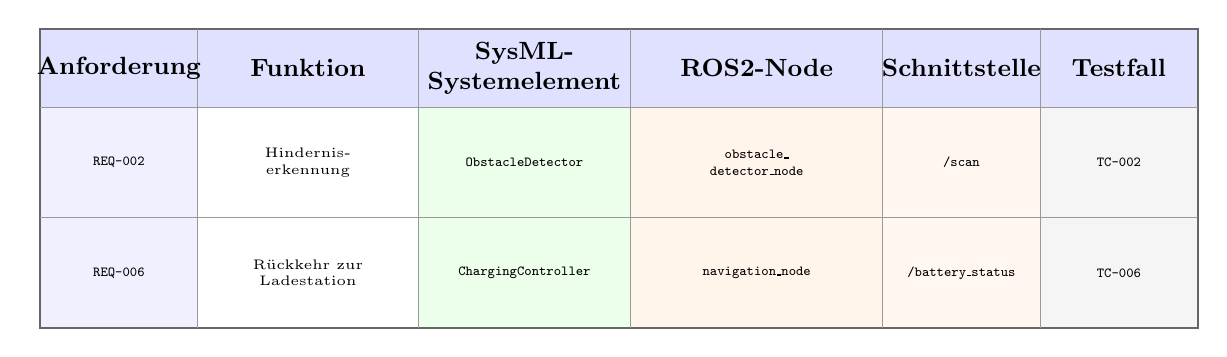
\begin{tikzpicture}[
    every node/.style={font=\small},
    x=1cm, y=1cm
]

% --- Spaltengrenzen (x) und Zeilengrenzen (y) in cm ---
% Spalten: Anforderung | Funktion | SysML-Systemelement | ROS2-Node | Schnittstelle | Testfall
% x0=0, x1=2.0, x2=4.8, x3=7.5, x4=10.7, x5=12.7, x6=14.7
% Zeilen (von oben): y0=3.8 (Kopf oben), y1=2.8 (Kopf unten / Zeile1 oben),
%                     y2=1.4 (Zeile1 unten / Zeile2 oben), y3=0 (Zeile2 unten)

% --- Spaltenhintergrund fuer Datenzeilen (y3 bis y1) ---
\fill[blue!6]   (0,0)    rectangle (2.0,2.8);
\fill[white]    (2.0,0)  rectangle (4.8,2.8);
\fill[green!8]  (4.8,0)  rectangle (7.5,2.8);
\fill[orange!8] (7.5,0)  rectangle (10.7,2.8);
\fill[orange!6] (10.7,0) rectangle (12.7,2.8);
\fill[black!4]  (12.7,0) rectangle (14.7,2.8);

% --- Kopfzeile ueberdeckend einfaerben ---
\fill[blue!12] (0,2.8) rectangle (14.7,3.8);

% --- Rasterlinien: Aussenrahmen ---
\draw[black!60, thick] (0,0) rectangle (14.7,3.8);

% --- Rasterlinien: senkrechte Spaltentrenner ---
\draw[black!40] (2.0,0)  -- (2.0,3.8);
\draw[black!40] (4.8,0)  -- (4.8,3.8);
\draw[black!40] (7.5,0)  -- (7.5,3.8);
\draw[black!40] (10.7,0) -- (10.7,3.8);
\draw[black!40] (12.7,0) -- (12.7,3.8);

% --- Rasterlinien: waagrechte Zeilentrenner ---
\draw[black!40] (0,1.4) -- (14.7,1.4);
\draw[black!40] (0,2.8) -- (14.7,2.8);

% --- Kopfzeilentext ---
\node[font=\small\bfseries] at (1.0,3.3)  {Anforderung};
\node[font=\small\bfseries] at (3.4,3.3)  {Funktion};
\node[font=\small\bfseries, align=center] at (6.15,3.3) {SysML-\\Systemelement};
\node[font=\small\bfseries] at (9.1,3.3)  {ROS2-Node};
\node[font=\small\bfseries] at (11.7,3.3) {Schnittstelle};
\node[font=\small\bfseries] at (13.7,3.3) {Testfall};

% --- Zeile 1: REQ-002 ---
\node[font=\tiny] at (1.0,2.1)  {\texttt{REQ-002}};
\node[font=\tiny, align=center] at (3.4,2.1)  {Hindernis-\\erkennung};
\node[font=\tiny] at (6.15,2.1) {\texttt{ObstacleDetector}};
\node[font=\tiny, align=center] at (9.1,2.1)  {\texttt{obstacle\_}\\\texttt{detector\_node}};
\node[font=\tiny] at (11.7,2.1) {\texttt{/scan}};
\node[font=\tiny] at (13.7,2.1) {\texttt{TC-002}};

% --- Zeile 2: REQ-006 ---
\node[font=\tiny] at (1.0,0.7)  {\texttt{REQ-006}};
\node[font=\tiny, align=center] at (3.4,0.7)  {Rückkehr zur\\Ladestation};
\node[font=\tiny] at (6.15,0.7) {\texttt{ChargingController}};
\node[font=\tiny] at (9.1,0.7)  {\texttt{navigation\_node}};
\node[font=\tiny] at (11.7,0.7) {\texttt{/battery\_status}};
\node[font=\tiny] at (13.7,0.7) {\texttt{TC-006}};

\end{tikzpicture}

